\section{Resultats} 

Le premier résultat à remarquer est l'inclusion du support pour le \textit{TC37xEXT} dans la version 3.8.11 de l'aurix toolbox en python et hipersim. 

Le switch Marvell a été modélisé pour initialiser les ports dans le logiciel AUTOSAR mais ce développement a pris plus de temps que l'attendu parce que les datasheets du fournisseur sont arrivées en retard. En autre, toolbox Ethernet\footnote{Toolbox développé par la division australienne de la société.} ne supportait pas certains types de protocole et les instructions arrivaient incomplets dans le switch. Le protocole Clause 22 utilis\'e dans le bus MDIO c'était un nouveau protocole qui a pris du temps à être développé.  

En arrivant à la fin du projet l'aurix encore à des problèmes parce qu'il cherche à se communiquer avec des transceivers \`a travers du switch. La solution propos\'e pour ces composants, vu que ce sont des composant qui se communiquent \`a travers du switch, c'était faire une machine \`a état qui répond le nécessaire pour initialiser les ports Ethernet mais c'est encore en développement et c'est un procès qui peut générer des problèmes au futur. 

Le premier cas d'utilisation a suivi le chemin des données de la figure \ref{fig:autosar-com-stack} : \textit{Microcontroler} $->$ \textit{CAN\_Driver} $->$ \textit{CAN\_IF} $->$ \textit{PDU-R} $->$ \textit{SocketAdapter}\cite{sock_adp_man} $->$ \textit{DETError}\cite{det_man}. Dans le \textit{SocketAdapter} le logiciel trouve un problème parce que les connections ne sont pas initialises. Ce problème des ports touche aussi le deuxième cas d'utilisation donc cela n'a pas pu être test\'e. 

\begin{figure}[!htb] 
\centering 
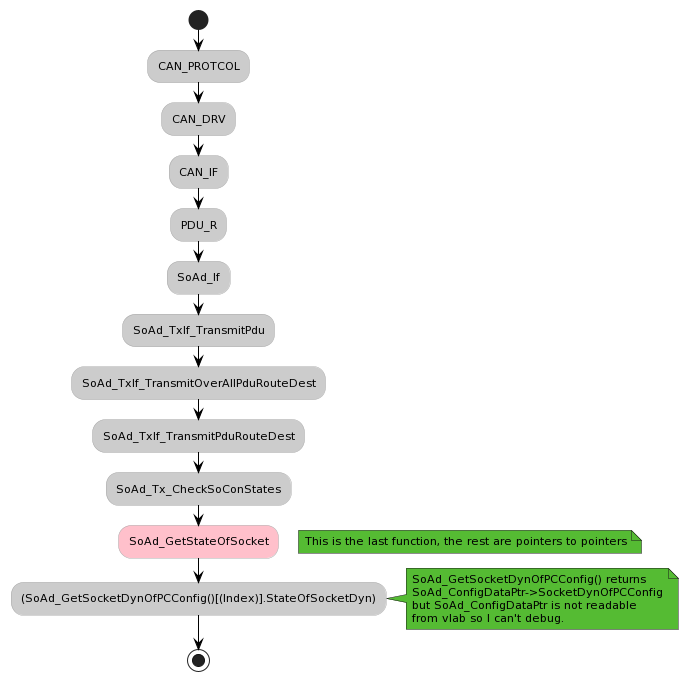
\includegraphics[width=\textwidth]{img/SoAd_Error.png} 
\caption{Socket adaptor error} 
\label{fig:soad-error} 
\end{figure}
